\section{System Architecture}
\label{sec:arch}

LogChirpy is built on React Native / Expo SDK~52 targeting Android (API\,29+) and
iOS.
Three service pillars — ML Processing, BirDex Encyclopedia, and Logging System —
share a common navigation shell built on Expo Router (Figure~\ref{fig:arch}).
All ML inference runs locally via \texttt{react-native-fast-tflite};
network access is limited to optional Firestore sync and first-run image download.

\begin{figure*}[t]
  \centering
  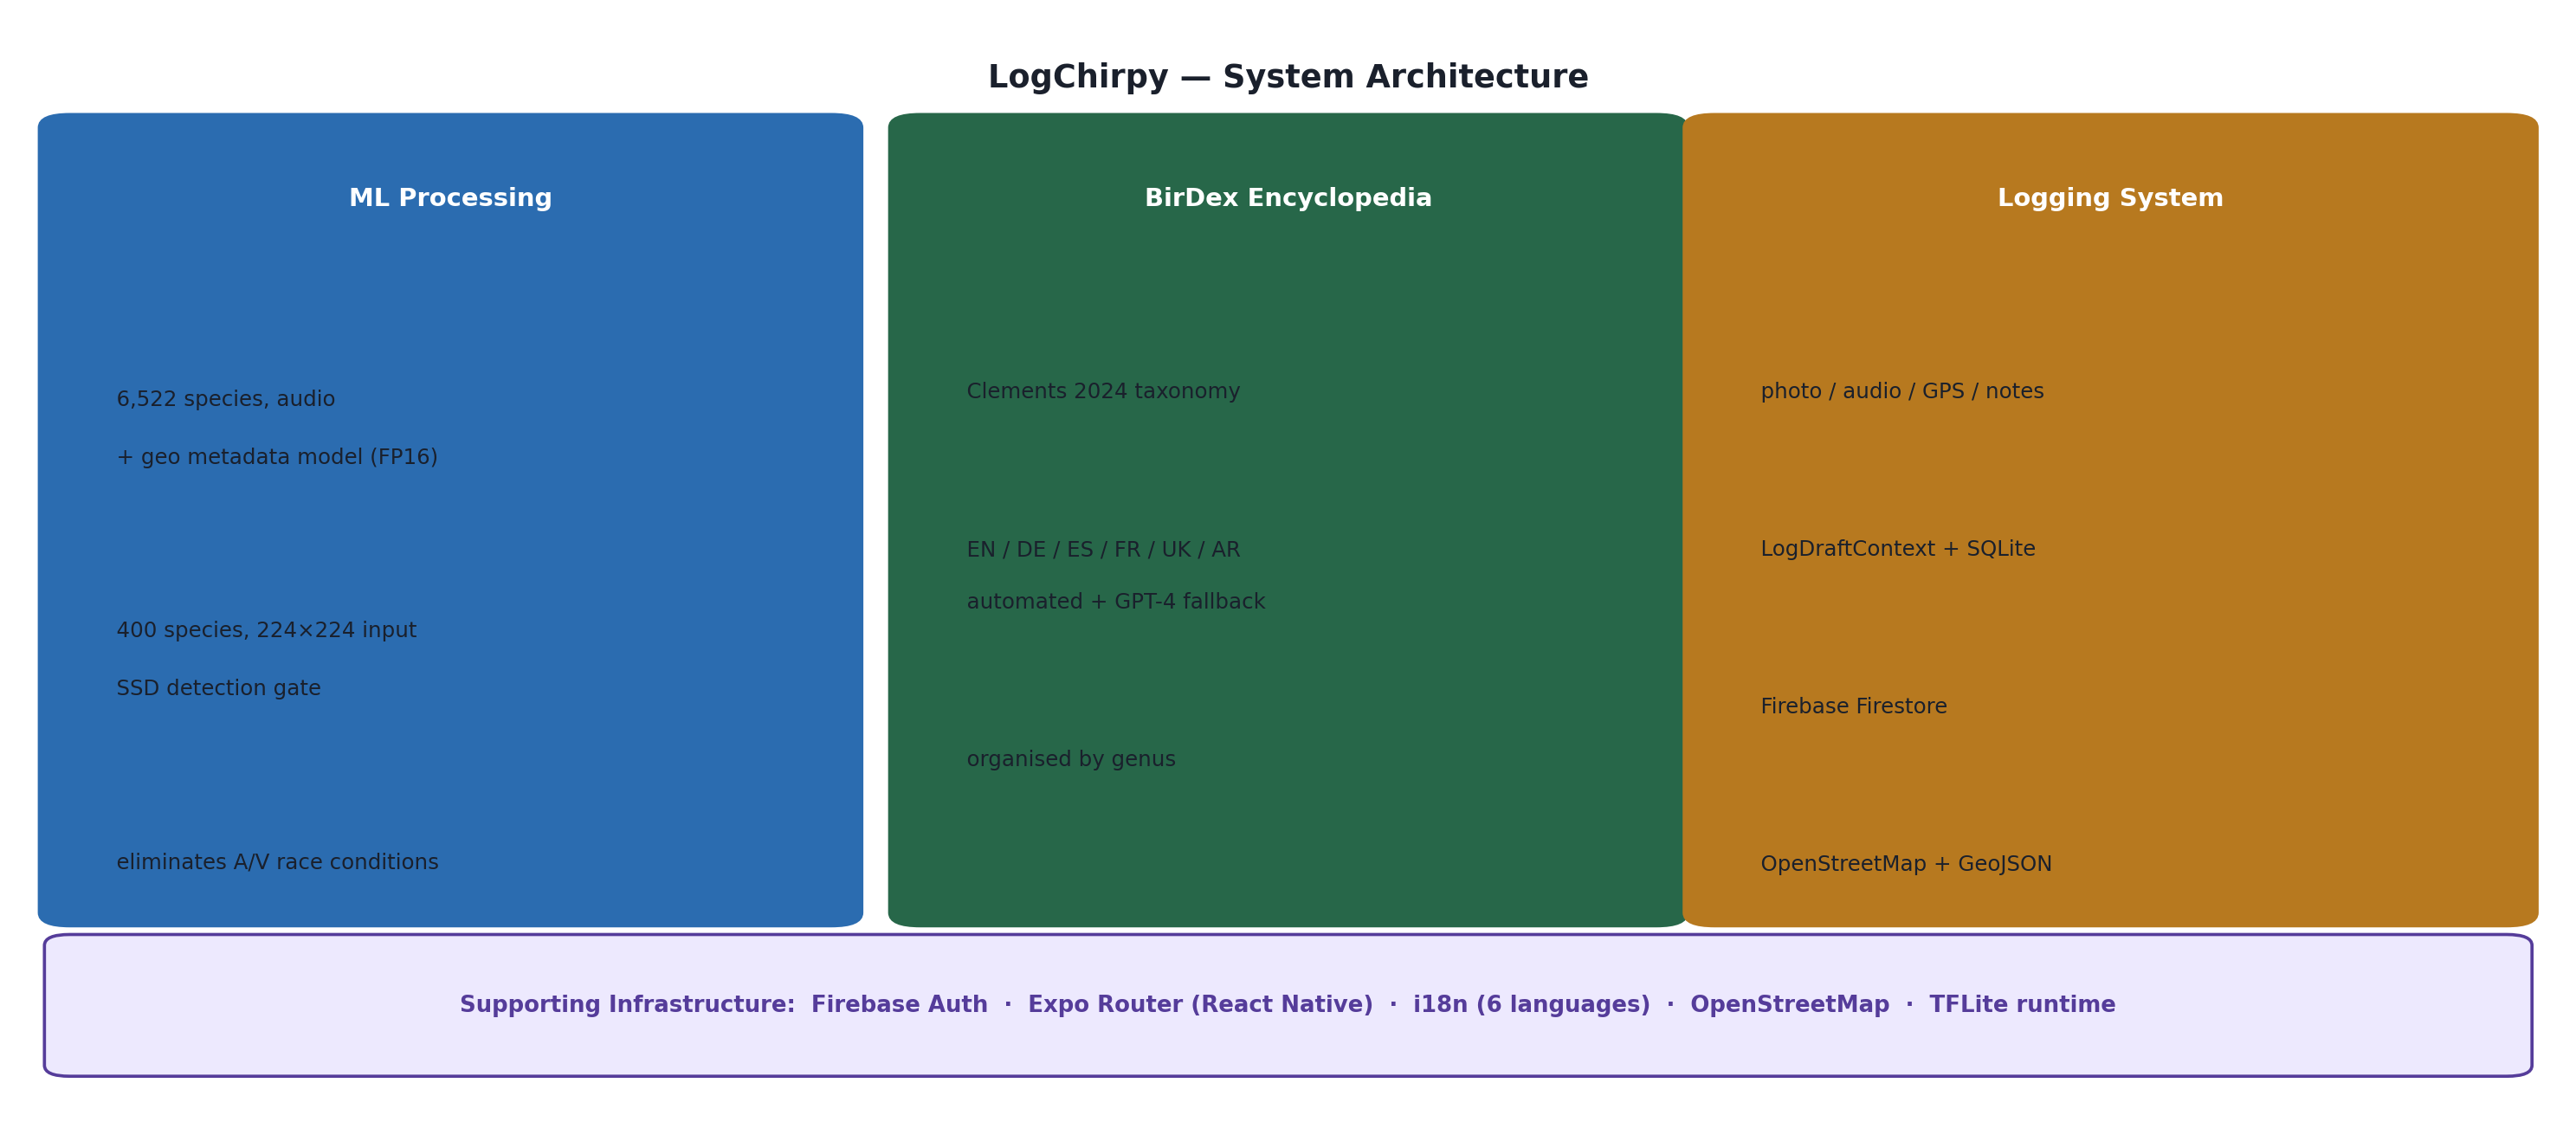
\includegraphics[width=\linewidth]{img/architecture.png}
  \caption{Three-pillar architecture. Each pillar is functionally independent;
           the unified sequential ML pipeline service (bottom bar) orchestrates
           audio and image processing to prevent Android file-lock conflicts.}
  \label{fig:arch}
\end{figure*}

\subsection{Audio Pipeline}

BirdNET\,v2.4~\cite{BirdNET2021} is implemented via two sequential TFLite models
(Figure~\ref{fig:pipelines}).
Audio is captured at 48\,kHz mono; a 150–15\,000\,Hz bandpass filter attenuates
wind and handling noise and the signal is normalised to $[-1,1]$.
The \textbf{acoustic model} (FP32) accepts a $\mathbb{R}^{1\times144\,000}$
tensor and outputs sigmoid logits over 6,522 species.
When GPS is available the \textbf{metadata model} (FP16) takes
$[\text{lat},\,\text{lon},\,\text{week-cos}]$ and produces a geographic prior;
scores are fused as
\begin{equation}
  p_{\text{blend}} = p_{\text{audio}}\cdot(0.7 + 0.3\cdot p_{\text{geo}}),
  \label{eq:blend}
\end{equation}
following the whoBIRD reference implementation~\cite{WhoBird2023}.

\subsection{Image Pipeline}

Camera frames are JPEG-compressed (quality\,0.3) and passed to an SSD MobileNet
V1 detection gate (MLKit).
Frames without a sufficiently confident bird detection are discarded.
Passing frames go to \texttt{bird\_classifier\_metadata.tflite}
(MobileNetV2~\cite{Sandler2018}): input $\mathbb{R}^{1\times224\times224\times3}$
normalised to $[-1,1]$, output softmax logits over 400 species.

\textbf{Sequential lock.}
Concurrent audio recording and camera processing caused
\texttt{MediaRecorder} file-lock conflicts on Android.
\texttt{unifiedMLPipelineService.ts} enforces image-before-audio sequencing,
eliminating all recorded stability errors.

\begin{figure*}[t]
  \centering
  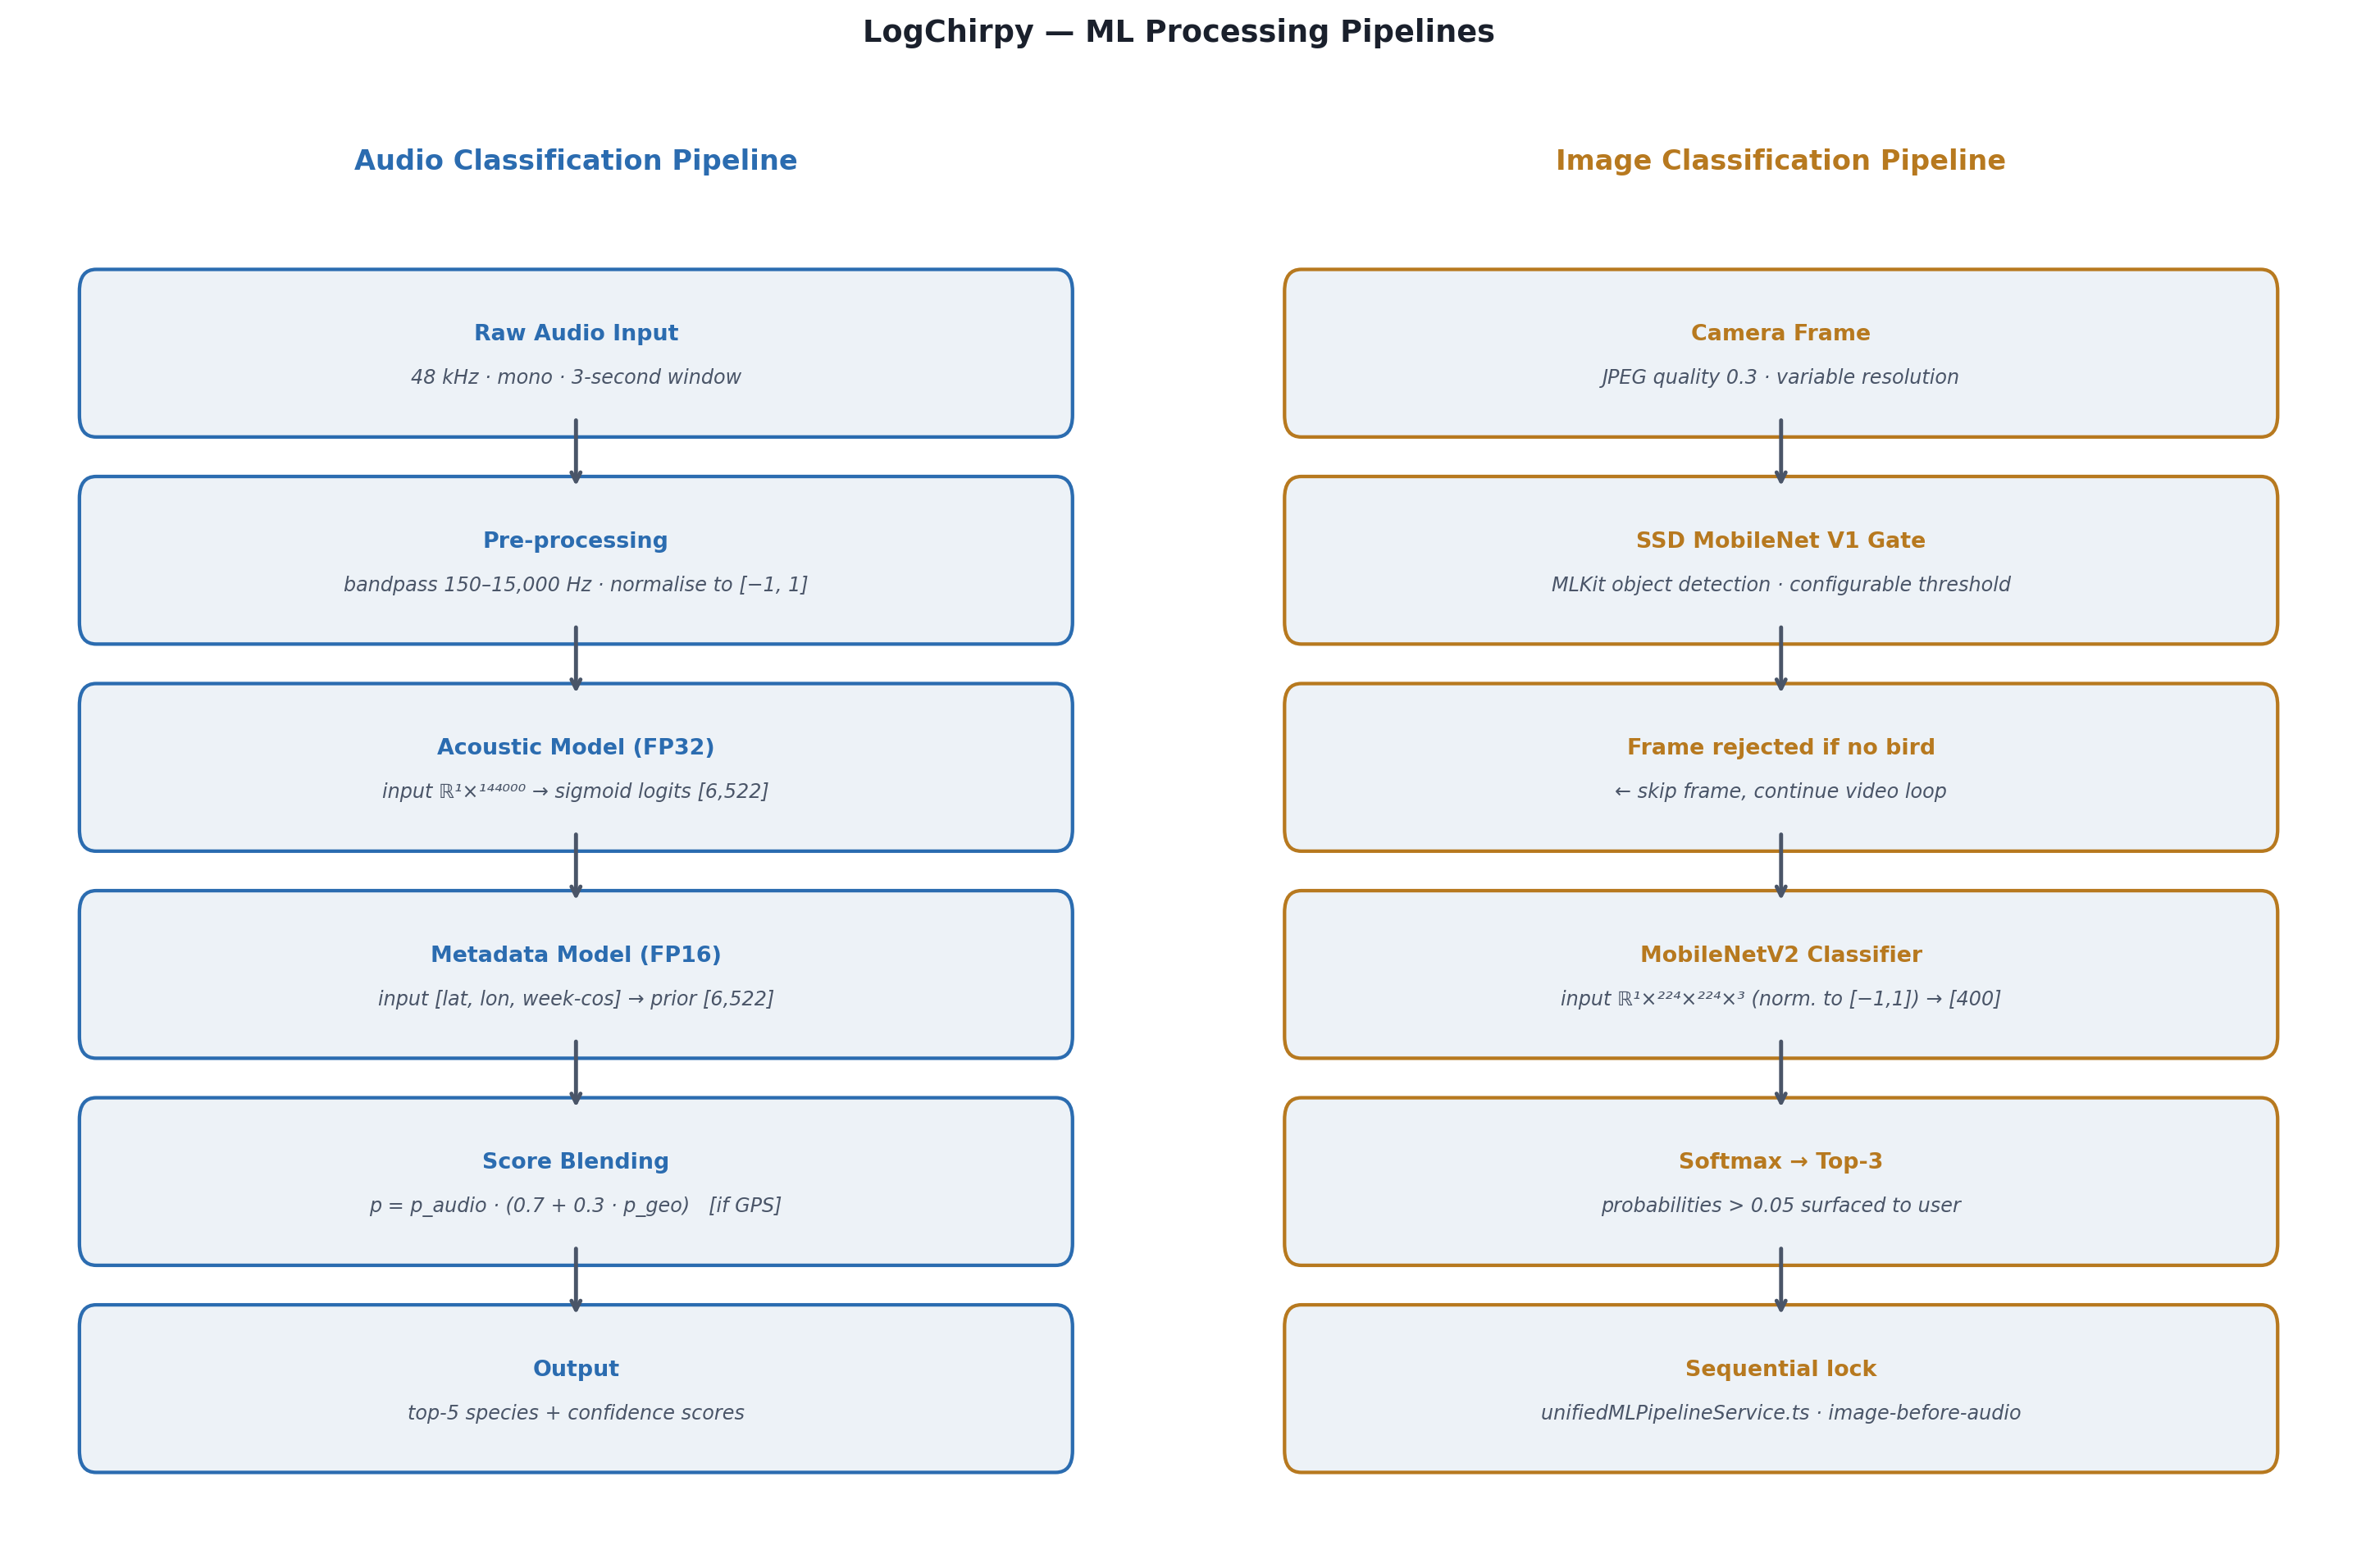
\includegraphics[width=\linewidth]{img/pipelines.png}
  \caption{Audio (left) and image (right) ML pipelines with tensor shapes.
           Both run entirely on-device via TFLite; the sequential lock prevents
           concurrent audio/camera conflicts on Android.}
  \label{fig:pipelines}
\end{figure*}

\subsection{BirDex Encyclopedia}

BirDex stores the complete Clements 2024 checklist~\cite{Clements2024} in an
on-device SQLite database (Table~\ref{tab:schema}).
Translations across six languages were generated by an automated pipeline
(DeepL\,$\to$\,Google Translate\,$\to$\,GPT-4 fallback) and spot-checked by
family.
Reference images (9,331 WebP files, $\approx$50\,kB each) are downloaded from
Wikimedia Commons at first launch and cached by Clements genus.

\begin{table}[htb]
\centering
\small
\setlength{\tabcolsep}{4pt}
\begin{tabular}{lll}
\hline
\textbf{Column} & \textbf{Type} & \textbf{Description} \\
\hline
\texttt{species\_code}    & TEXT PK & eBird 6-letter code \\
\texttt{english\_name}    & TEXT    & Clements English name \\
\texttt{scientific\_name} & TEXT    & Binomial nomenclature \\
\texttt{family / order}   & TEXT    & Clements taxonomy \\
\texttt{range}            & TEXT    & Breeding/wintering range \\
\texttt{de/es/fr/uk/ar}   & TEXT    & Translated names (×5) \\
\texttt{hasBeenLogged}    & INT     & Observation flag \\
\hline
\end{tabular}
\caption{BirDex SQLite schema (abridged, 33,241 rows).}
\label{tab:schema}
\end{table}
